\documentclass{ximera}

\usepackage{microtype}
\usepackage{tikz}
\usepackage{tkz-euclide}
\usetkzobj{all}
\tikzstyle geometryDiagrams=[ultra thick,color=blue!50!black]

\renewcommand{\epsilon}{\varepsilon}



\title{Lines in hyperbolic geometry}

\begin{document}
\begin{abstract}
Here we examine ``lines'' in hyperbolic geometry and prove a
hyperbolic version of the Pythagorean Theorem.
\end{abstract}
\maketitle

\subsection*{Hyperbolic coordinates, a shortest path from the North Pole}

We next will figure out what is the shortest path you can take between
two points in hyperbolic geometry. Since $K$ is negative, we must do
our calculation using only $(x,y,z)$-coordinates. However, this will
allow us to see the full power of working in $K$-warped space, since
our work will be essentially the same as when $K$ was positive---though
our parametrization will be different.
\begin{image}
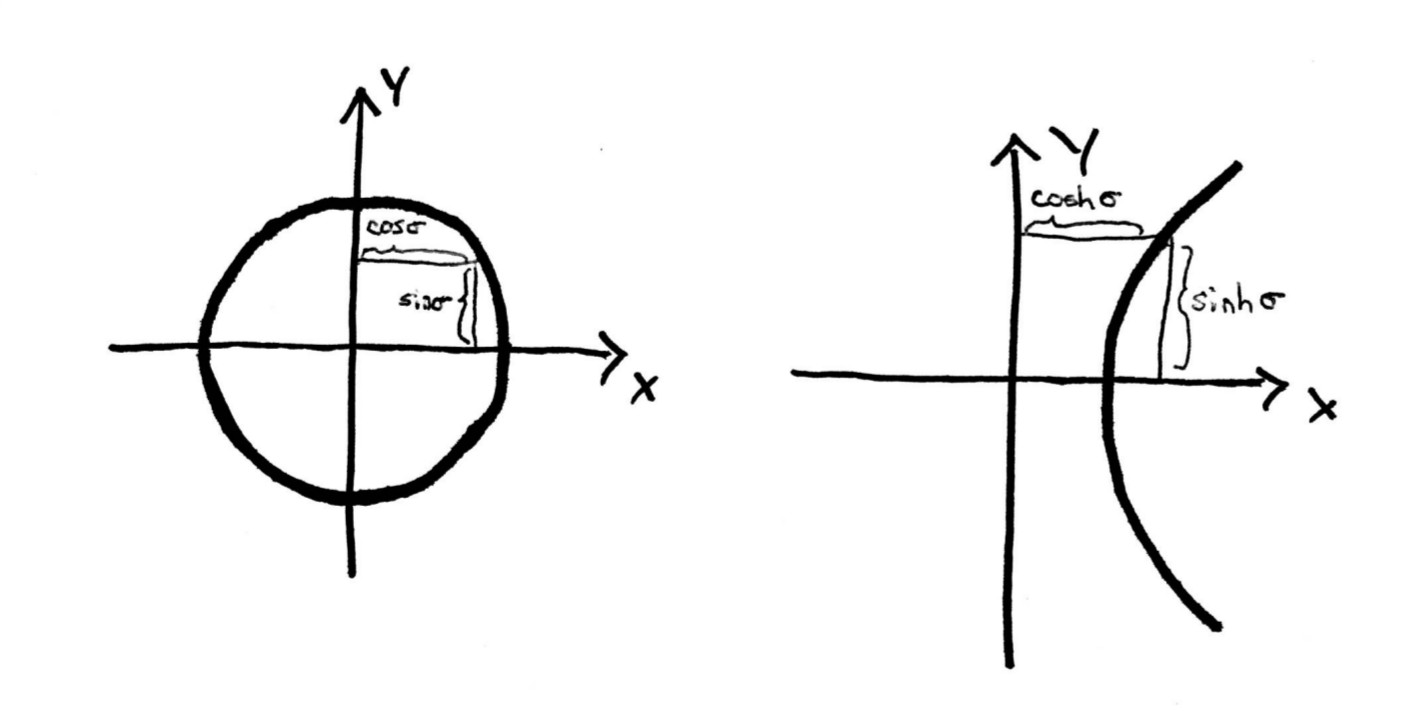
\includegraphics[width=4in]{trigVsHyp.jpg}
\end{image}


Just as $(\cos\sigma,\sin\sigma)$ parametrize the unit circle,
hyperbolic functions
\[
\left(
\cosh\sigma=\frac{e^{\sigma}+e^{-\sigma}}{2},
\sinh\sigma=\frac{e^{\sigma}-e^{-\sigma}}{2}
\right)
\]
parametrize the `unit' hyperbola. Hence we define
\begin{align*}
  x(\sigma,\tau) &=|K|^{-1/2}\cdot \sinh \sigma\cdot\cos \tau,\\
  y(\sigma,\tau) &=|K|^{-1/2}\cdot\sinh\sigma\cdot\sin \tau,\\
  z(\sigma,\tau) &=\cosh \sigma,
\end{align*}
where $0\le \sigma< \infty$ and $0\le \tau<2\pi$.

\begin{image}
  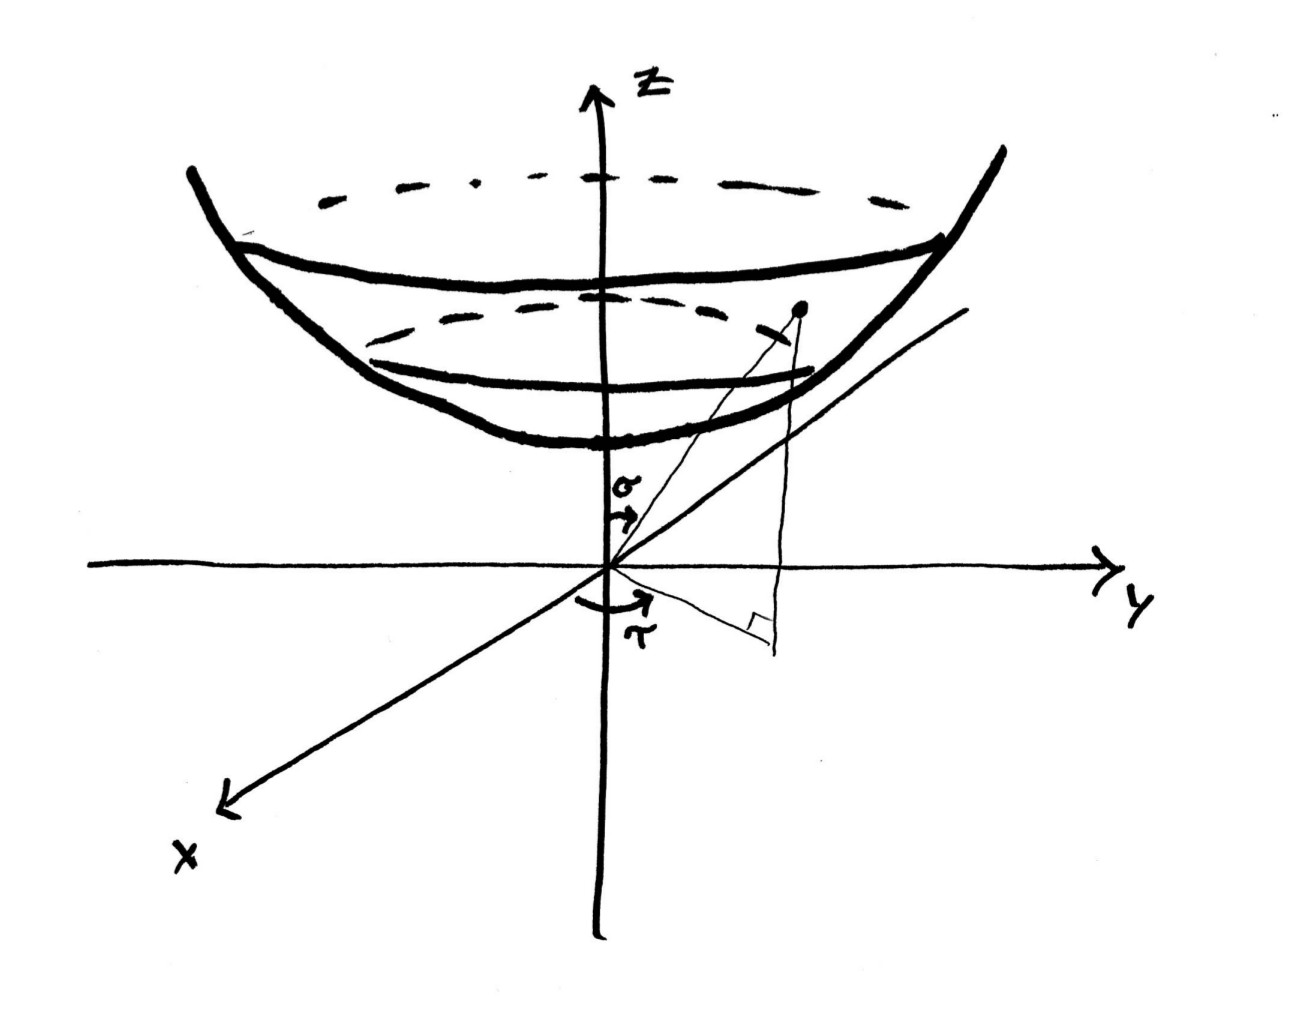
\includegraphics[width=3in]{hyperbolicPara.jpg}
\end{image}


\begin{problem}
Show that these hyperbolic coordinates do actually parametrize the
$K$-geometry.
\begin{hint}
  Remember, $K$ is negative.
\end{hint}
\begin{hint}
  Remember,
  \[
  -\sinh^2\sigma + \cosh^2\sigma =1.
  \]
\end{hint}
\begin{hint}
  This is an exercise in ``double-containment.'' To show the one
  direction, show
\[
K\left(x(\sigma,\tau)^{2}+y(\sigma,\tau)^{2}\right)+z(\sigma,\tau)^{2}
= 1
\]
for all $(\sigma,\tau)$. To show the other direction, appeal to the
diagram above.
\end{hint}
\begin{freeResponse}
  We will first show that the set determined by
  \[
  \left(x(\sigma,\tau), y(\sigma,\tau), z(\sigma,\tau)\right)
  \]
  lies on the surface
  \[
  K\left(x(\sigma,\tau) ^{2}+y(\sigma,\tau) ^{2}\right) +z(\sigma,\tau)^{2} = 1
  \]
  where $K<0$. Substituting we have
  $K\left(x(\sigma,\tau) ^{2}+y(\sigma,\tau) ^{2}\right)
  +z(\sigma,\tau)^{2}$
  \begin{align*}
    &=K\left((|K|^{-1/2}\cdot\sinh\sigma\cdot\cos\tau)^{2}+(|K|^{-1/2}\cdot\sinh\sigma\cdot\sin\tau)^{2}\right) +(\cosh\sigma)^{2} \\
    &= -\sinh^2\sigma\cdot\cos^2\tau-\sinh^2\sigma\sin^2\tau + \cosh^2\sigma \\
    &= -\sinh^2\sigma(\cos^2\tau+\sin^2\tau) + \cosh^2\sigma \\
    &= -\sinh^2\sigma + \cosh^2\sigma \\
    &=1.
  \end{align*}
  Now we must show that every point on the surface can be obtained from
  \[
  \left(x(\sigma,\tau), y(\sigma,\tau), z(\sigma,\tau)\right).
  \]
  We see this from the diagram above. 
\end{freeResponse}
\end{problem}

Just as we did on the $R$-sphere, we can write a path on the
$K$-surface by giving a path in the $(\sigma,\tau)$-plane. Again, we
will need to figure out the $K$-dot product in
$(\sigma,\tau)$-coordinates so that we can compute the lengths of
paths in these coordinates.


\begin{problem}
Suppose we have a curve $X$ in $K$-warped space that is a function of
a $\sigma(t)$ and $\tau(t)$. Use the chain rule to compute
\[
\dd[x]{t},\qquad \dd[y]{t}, \qquad \dd[z]{t},
\]
in terms of $\dd[\sigma]{t}$, $\dd[\tau]{t}$, $\pp[x]{\sigma}$,
$\pp[y]{\sigma}$, $\pp[z]{\sigma}$, $\pp[x]{\tau}$, $\pp[y]{\tau}$,
and $\pp[z]{\tau}$.
\begin{hint}
  Simply write down the answer from a previous problem.
\end{hint}
\begin{freeResponse}
  Write
  \begin{align*}
    \dd[x]{t} &= \pp[x]{\sigma}\cdot\dd[\sigma]{t}+\pp[x]{\tau}\cdot\dd[\tau]{t}, \\
    \dd[y]{t} &= \pp[y]{\sigma}\cdot\dd[\sigma]{t}+\pp[y]{\tau}\cdot\dd[\tau]{t}, \\
    \dd[z]{t} &= \pp[z]{\sigma}\cdot\dd[\sigma]{t}+\pp[z]{\tau}\cdot\dd[\tau]{t}.  
  \end{align*}
\end{freeResponse}
\end{problem}



\begin{problem}
  With the same setting as in the previous problem, rewrite the result
  of your computation in matrix notation to find $D_{\mathrm{hyp}}$ such
  that
\[
\begin{bmatrix}
\dd[x]{t} & \dd[y]{t} & \dd[z]{t}
\end{bmatrix}
=
\begin{bmatrix}
\frac{d\sigma}{dt} & \frac{d\tau}{dt}
\end{bmatrix}\cdot D_{\mathrm{hyp}}
\]
in terms of $\pp[x]{\sigma}$, $\pp[y]{\sigma}$, $\pp[z]{\sigma}$,
$\pp[x]{\tau}$, $\pp[y]{\tau}$, and $\pp[z]{\tau}$.
\begin{hint}
  Simply write down the answer from a previous problem.
\end{hint}
\begin{freeResponse}
  \[
  D_{\mathrm{hyp}} =
  \begin{bmatrix}
    \pp[x]{\sigma} & \pp[y]{\sigma} & \pp[z]{\sigma} \\
    \pp[x]{\tau}   & \pp[y]{\tau}   & \pp[z]{\tau}
  \end{bmatrix}.
  \]
\end{freeResponse}
\end{problem}


\begin{problem}
  Now find $P_\mathrm{hyp}$ in terms of $K$, $\pp[x]{\sigma}$, $\pp[y]{\sigma}$,
  $\pp[z]{\sigma}$, $\pp[x]{\tau}$, $\pp[y]{\tau}$, and $\pp[z]{\tau}$
  such that
  \[
  \left(\dd[x]{t}, \dd[y]{t}, \dd[z]{t}\right)\bullet_K
  \left(\dd[x]{t}, \dd[y]{t}, \dd[z]{t}\right)
  =
  \begin{bmatrix}
    \dd[\sigma]{t} &  \dd[\tau]{t}
  \end{bmatrix}
  \cdot P_\mathrm{hyp}
  \cdot
  \begin{bmatrix}
    \dd[\sigma]{t} \\  \dd[\tau]{t}
  \end{bmatrix}.
  \]
  \begin{hint}
    Simply write down the answer from a previous problem.
  \end{hint}
  \begin{freeResponse}
    \[
    P_\mathrm{hyp} =
    \begin{bmatrix}
        \left(\pp[x]{\sigma}\right)^2 + \left(\pp[y]{\sigma}\right)^2 + \left(\pp[z]{\sigma}\right)^2K^{-1} & \pp[x]{\sigma}\pp[x]{\tau} + \pp[y]{\sigma}\pp[y]{\tau} + \pp[z]{\sigma}\pp[z]{\tau} K^{-1}\\
        \pp[x]{\sigma}\pp[x]{\tau} + \pp[y]{\sigma}\pp[y]{\tau} + \pp[z]{\sigma}\pp[z]{\tau} K^{-1}       & \left(\pp[x]{\tau}\right)^2 + \left(\pp[y]{\tau}\right)^2 + \left(\pp[z]{\tau}\right)^2K^{-1}
      \end{bmatrix}.
    \]
  \end{freeResponse}
\end{problem}




\begin{problem}
  Set
  \begin{align*}
    x(\sigma,\tau) &=|K|^{-1/2}\cdot \sinh\sigma\cdot \cos \tau,\\
    y(\sigma,\tau) &=|K|^{-1/2}\cdot \sinh\sigma\cdot \sin\tau,\\
    z(\sigma,\tau) &=\cosh\sigma,
  \end{align*}
  and show that $P_\mathrm{hyp}$ from the problem above is
  \[
  P_\mathrm{hyp} =
  \begin{bmatrix}
    |K|^{-1} & 0 \\
    0 &  |K|^{-1}\cdot\sinh^2 \sigma
  \end{bmatrix}.
  \]
  \begin{freeResponse}
    Write
    \[
    \begin{split}
      \pp[x]{\sigma} &= |K|^{-1/2}\cdot \cosh\sigma\cdot \cos \tau, \\
      \pp[y]{\sigma} &= |K|^{-1/2}\cdot \cosh\sigma\cdot \sin\tau,\\
      \pp[z]{\sigma} &= \sinh\sigma,
    \end{split}
    \qquad
    \begin{split}
      \pp[x]{\tau} &= -|K|^{-1/2}\cdot \sinh\sigma\cdot \sin \tau,\\
      \pp[y]{\tau} &= |K|^{-1/2}\cdot \sinh\sigma\cdot \cos\tau,\\
      \pp[z]{\tau} &= 0. 
    \end{split}
    \]
    Now we see $\left(\pp[x]{\sigma}\right)^2 + \left(\pp[y]{\sigma}\right)^2 + \left(\pp[z]{\sigma}\right)^2K^{-1}$
    \begin{align*}
      &= \left(|K|^{-1/2}\cdot \cosh\sigma\cdot \cos \tau \right)^2 + \left(|K|^{-1/2}\cdot \cosh\sigma\cdot \sin\tau\right)^2 + \left(\sinh\sigma\right)^2K^{-1}\\
      &= |K|^{-1}\cdot \cosh^2\sigma\cdot \cos^2 \tau + |K|^{-1}\cdot \cosh^2\sigma\cdot \sin^2\tau - |K|^{-1} \sinh^2\sigma \\
      &= |K|^{-1}\cdot \cosh^2\sigma\left(\cos^2 \tau + \sin^2\tau\right) -|K|^{-1} \sinh^2\sigma \\
      &= |K|^{-1}\left(\cosh^2\sigma -\sinh^2\sigma\right) \\
      &= |K|^{-1}.
    \end{align*}
    That $\pp[x]{\sigma}\pp[x]{\tau} + \pp[y]{\sigma}\pp[y]{\tau} + \pp[z]{\sigma}\pp[z]{\tau} K^{-1}$
    \begin{align*}
      &= -|K|^{-1}\cdot \cos\sigma\cdot \cos \tau \cdot \sin\sigma\cdot \sin \tau + |K|^{-1}\cdot \cos\sigma\cdot \cos \tau \cdot \sin\sigma\cdot \sin \tau\\
      &= 0.
    \end{align*}
    And finally that $\left(\pp[x]{\tau}\right)^2 + \left(\pp[y]{\tau}\right)^2 + \left(\pp[z]{\tau}\right)^2K^{-1}$
     \begin{align*}
       &= \left(|K|^{-1/2}\cdot \sinh\sigma\cdot \sin \tau \right)^2 + \left( |K|^{-1/2}\cdot \sinh\sigma\cdot \cos\tau \right)^2 \\
       &= |K|^{-1}\cdot \sinh^2\sigma\cdot \sin^2 \tau + |K|^{-1}\cdot \sinh^2\sigma\cdot \cos^2\tau \\
       &= |K|^{-1}\cdot \sinh^2\sigma\left(\sin^2 \tau + \cos^2\tau\right) \\
       &= |K|^{-1}\cdot \sinh^2\sigma.
     \end{align*}
     Hence
     \[
     P_\mathrm{hyp} =
  \begin{bmatrix}
    |K|^{-1} & 0 \\
    0 & |K|^{-1}\cdot\sinh^2 \sigma
  \end{bmatrix}.
     \]
  \end{freeResponse}
\end{problem}



\begin{definition}
  Let $V_\mathrm{hyp}$ and $W_\mathrm{hyp}$ be a vectors in
  $(\sigma,\tau)$-coordinates originating at the same
  $(\sigma,\tau)$-coordinate. Define
  \[
  V_\mathrm{hyp} \bullet_\mathrm{hyp} W_\mathrm{hyp} = V_\mathrm{hyp} \cdot P_\mathrm{hyp} \cdot W_\mathrm{hyp}^\transpose
  \]
  where
  \[
     P_\mathrm{hyp} =
  \begin{bmatrix}
    |K|^{-1} & 0 \\
    0 & |K|^{-1}\cdot\sinh^2 \sigma
  \end{bmatrix}
  \]
  and $\sigma$ is determined by the coordinate that the vectors
  originate from.
\end{definition}



Now notice that you can write a path on the $K$-surface by giving a
path $\left( \sigma(t),\tau(t)\right)$ in the
$(\sigma,\tau)$-plane. In fact, you can use $\sigma$ as the parameter,
and just write
\[
\left(\sigma,\tau(\sigma)\right)
\]
where $\tau$ is a function of $\sigma$. To write a path that starts at
the North Pole, just write
\[
\left(\sigma,\tau(\sigma)\right), \qquad 0\leq\sigma\leq\varepsilon
\]
and demand that
\[
\tau(0) =0.
\]
If you want the path to end on the plane $y=\hat{y}=0$, demand
additionally that
\[
\tau(\varepsilon) =0.
\]


 Now given a path on the $K$-surface
 \[
 \left(\sigma,\tau(\sigma)\right),\qquad0\leq\sigma \leq\varepsilon
 \]
 with
 \[
 \tau\left(  0\right)  =0.
 \]
 and%
 \[
 \tau\left(  \varepsilon\right)  =0
 \]
 its length is given by the formula%
\[
L=\int_{0}^{\varepsilon} \sqrt{\left(1,\dd[\tau]{\sigma}\right)\bullet_\mathrm{hyp} \left(1,\dd[\tau]{\sigma}\right)}\d\sigma.
\]

\begin{problem}
  Prove that the shortest path on the $K$-surface from the North Pole
  \[
  N=\left( |K|^{-1/2}\cdot \sinh 0\cdot  \cos 0,|K|^{-1/2}\cdot \sinh  0\cdot \sin 0,\cosh
  0\right)
  \]
  to a point
  \[
  (x,y,z)=\left(|K|^{-1/2}\cdot \sinh \varepsilon,0,\cosh \varepsilon\right)
  \]
  is the path lying in the plane $y=0$.
  \begin{hint}
    Note that the following expression is always positive:
    \[
    1+\sinh^{2}\sigma\cdot \left(\frac{d\tau }{d\sigma}\right)^{2}.
    \]
    When is it minimal?
  \end{hint}

  \begin{freeResponse}
    Write
    \begin{align*}
    L  &=\int_{0}^{\varepsilon} \sqrt{\left(1,\dd[\tau]{\sigma}\right)\bullet_\mathrm{hyp} \left(1,\dd[\tau]{\sigma}\right)}\d\sigma\\
    &= \int_{0}^{\varepsilon} \sqrt{
      \begin{bmatrix} 1 & \dd[\tau]{\sigma}
      \end{bmatrix} \cdot P_\mathrm{hyp}\cdot
      \begin{bmatrix} 1 & \dd[\tau]{\sigma}
      \end{bmatrix}^\transpose}\d\sigma \\
    &= \int_{0}^{\varepsilon} \sqrt{
      \begin{bmatrix} 1 & \dd[\tau]{\sigma}
      \end{bmatrix}
      \begin{bmatrix}
        |K|^{-1} & 0 \\
        0 & |K|^{-1}\cdot\sinh^2 \sigma
      \end{bmatrix}
      \begin{bmatrix} 1 \\ \dd[\tau]{\sigma}
    \end{bmatrix}}\d\sigma \\
    &= \int_{0}^{\varepsilon} \sqrt{
      |K|^{-1}+|K|^{-1}\sinh^{2}\sigma\cdot \left(\frac{d\tau }{d\sigma}\right)^{2}
    }\d\sigma \\
    &= |K|^{-1/2}\int_{0}^{\varepsilon} \sqrt{
      1+\sinh^{2}\sigma\cdot \left(\frac{d\tau }{d\sigma}\right)^{2}
    }\d\sigma.
    \end{align*}
   Since $\sinh^{2}\sigma$ is is positive for almost all $\sigma\in[
     0,\varepsilon] $, $L$ is minimal only when
   $\frac{d\tau}{d\sigma}$ is identically $0$. But this means that
   $\tau\left( \sigma\right) $ is a constant function. Since
   $\tau\left( 0\right) =0$, this means that $\tau\left( \sigma\right)
   $ is identically $0$. Hence our path is determined by
   \begin{align*}
     x(\sigma,\tau) &=|K|^{-1/2}\cdot \sinh\sigma,\\
     y(\sigma,\tau) &=0,\\
     z(\sigma,\tau) &=\cosh \sigma,
   \end{align*}
   and this corresponds to a hyperbolic path embedded in the plane
   $y=\hat{y}=0$.
  \end{freeResponse}

\end{problem}








\section{Shortest path between any two points}

Just as we proved in spherical geometry that the shortest path is the
path cut out by
\[
K\left(  x^{2}+y^{2}\right)  +z^{2}=1
\]
and the plane containing the origin and the two points in question, we
will see that a completely analogous result is true in hyperbolic
geometry. Before we start, we will need one more class of rigid
motions to add to our collection.


\begin{problem}
  Assuming $K$ is negative, show
  \[
  N_\psi=
  \begin{bmatrix}
    \cosh\psi & 0 & |K|^{1/2}\cdot\sinh\psi\\
    0 & 1 & 0\\
    |K|^{-1/2}\cdot\sinh\psi & 0 & \cosh\psi
  \end{bmatrix}.
  \]
  is a $K$-rigid motion.
  \begin{freeResponse}
    We will show that $N_\psi$ is $K$ orthogonal. Write
    \[
    N_\psi
      \begin{bmatrix}
        1 & 0 & 0 \\
        0 & 1 & 0 \\
        0 & 0 & K^{-1}
      \end{bmatrix}
      N_\psi^\transpose
    \]
    \begin{align*}
  &=
      \begin{bmatrix}
    \cosh\psi & 0 & |K|^{1/2}\cdot\sinh\psi\\
    0 & 1 & 0\\
    |K|^{-1/2}\cdot\sinh\psi & 0 & \cosh\psi
      \end{bmatrix}
      \begin{bmatrix}
        1 & 0 & 0 \\
        0 & 1 & 0 \\
        0 & 0 & K^{-1}
      \end{bmatrix}
 \begin{bmatrix}
    \cosh\psi & 0 & |K|^{-1/2}\cdot\sinh\psi\\
    0 & 1 & 0\\
    |K|^{1/2}\cdot\sinh\psi & 0 & \cosh\psi
 \end{bmatrix} \\
&=\begin{bmatrix}
    \cosh\psi & 0 & -|K|^{-1/2}\cdot\sinh\psi\\
    0 & 1 & 0\\
    |K|^{-1/2}\cdot\sinh\psi & 0 &  K^{-1}\cosh\psi
      \end{bmatrix}
 \begin{bmatrix}
    \cosh\psi & 0 & |K|^{-1/2}\cdot\sinh\psi\\
    0 & 1 & 0\\
    |K|^{1/2}\cdot\sinh\psi & 0 & \cosh\psi
 \end{bmatrix}\\
&=\begin{bmatrix}
    \cosh^2\psi -\sinh^2\psi & 0 & |K|^{-1/2}\cdot\cosh\psi\cdot\sinh\psi- |K|^{-1/2}\cdot\cosh\psi\cdot\sinh\psi\\
    0 & 1 & 0\\
    |K|^{-1/2}\cdot\cosh\psi\cdot\sinh\psi- |K|^{-1/2}\cdot\cosh\psi\cdot\sinh\psi & 0 &  K^{-1}(\cosh^2\psi -\sinh^2\psi )
 \end{bmatrix}\\
 &=\begin{bmatrix}
        1 & 0 & 0 \\
        0 & 1 & 0 \\
        0 & 0 & K^{-1}
      \end{bmatrix}.
    \end{align*}
    Hence $N_\psi$ is $K$-orthogonal.
  \end{freeResponse}
\end{problem}







\begin{problem}
  Assuming $K$ is negative, consider
  \[
  N_\psi=
  \begin{bmatrix}
    \cosh\psi & 0 & |K|^{1/2}\cdot\sinh\psi\\
    0 & 1 & 0\\
    |K|^{-1/2}\cdot\sinh\psi & 0 & \cosh\psi
  \end{bmatrix}.
  \]
  Can you describe geometrically what this mapping is doing to the
  points in $K$-warped space?
  \begin{freeResponse}
    This rigid motion ``rotates'' along the $K$-surface around the $y$-axis:
    \begin{image}
      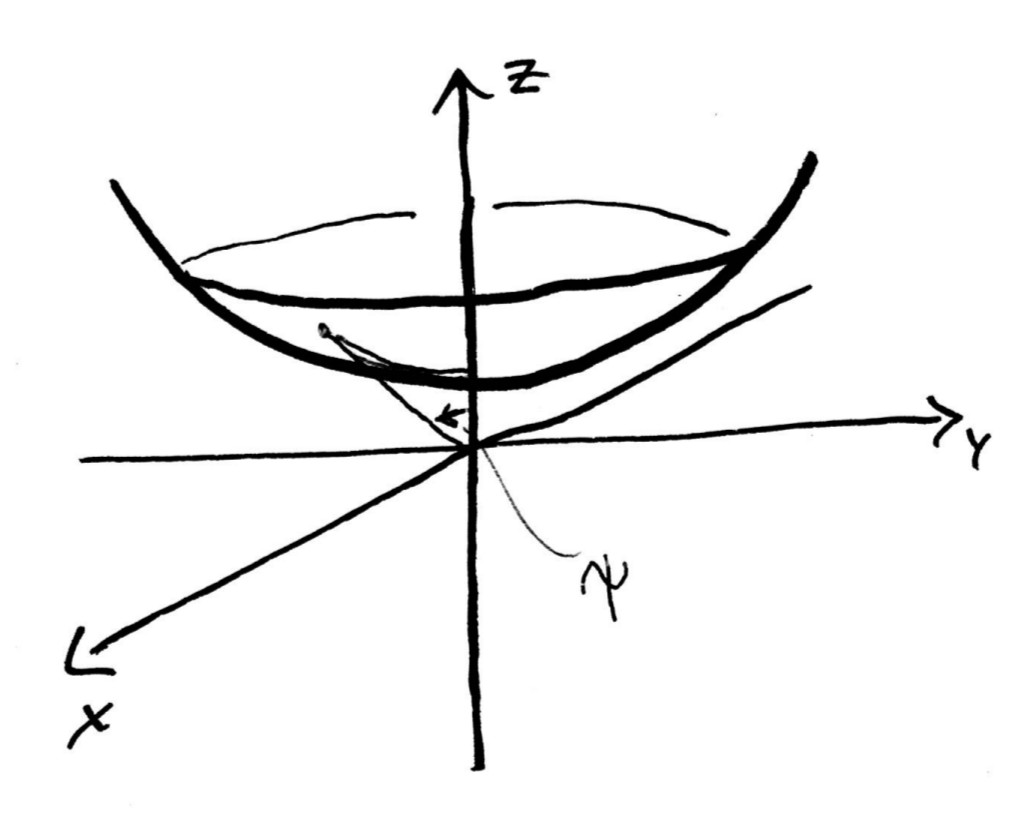
\includegraphics[width=3in]{hyperRigidMotion.jpg}
    \end{image}
  \end{freeResponse}
\end{problem}


\begin{theorem}
Given any two points $X_{1}=\left(x_{1},y_{1},z_{1}\right) $ and
$X_{2}=\left(x_{2},y_{2},z_{_{2}}\right) $ in $K$-geometry, the
shortest path between the two points is the path cut out by the set
\[
K\left(  x^{2}+y^{2}\right)  +z^{2}=1
\]
and the plane containing $(0,0,0)$, $X_{1}$, and $X_{2}$.
\end{theorem}


\begin{problem}
  Explain in words, with pictures as needed, how to prove this theorem
  by using the $K$-rigid motions
  \[
  M_\theta=
  \begin{bmatrix}
    \cos\theta & \sin\theta & 0\\
    -\sin\theta & \cos\theta & 0\\
    0 & 0 & 1
  \end{bmatrix}
  \qquad\text{and}\qquad
  N_\psi=
  \begin{bmatrix}
    \cosh\psi & 0 & |K|^{1/2}\cdot\sinh\psi\\
    0 & 1 & 0\\
    |K|^{-1/2}\cdot\sinh\psi & 0 & \cos\psi
  \end{bmatrix}.
  \]
  \begin{hint}
    $M_\theta$ is a $K$-rigid motion that rotates around the $z$-axis
    and $N_\psi$ is a $K$-rigid motion that ``rotates'' along the
    $K$-surface around the $y$-axis.
  \end{hint}
  \begin{hint}
    You should apply \textit{two} $K$-rigid motions of the form
    $M_\theta$ (for different angles) and one $K$-rigid motion of the
    form $N_\psi$---though not necessarily in that order!
  \end{hint}
  \begin{freeResponse}
    Given $X_1$ and $X_2$, we may instead consider $X_1\cdot M_\theta$
    and $X_2\cdot M_\theta$ where $\theta$ is chosen so that $X_1\cdot
    M_\theta$ is in the plane $y=0$.

    Next consider $X_1\cdot M_\theta\cdot N_\psi$ and $X_2\cdot
    M_\theta\cdot N_\psi$ where $\psi$ is chosen so that $X_1\cdot
    M_\theta\cdot N_\psi$ is at the North Pole.

    Finally consider $X_1\cdot M_\theta\cdot N_\psi\cdot M_\varphi$
    and $X_2\cdot M_\theta\cdot N_\psi\cdot M_\varphi$ where $\varphi$
    is chosen so that $X_1\cdot M_\theta\cdot N_\psi\cdot M_\varphi$
    is at the North Pole and $X_2\cdot M_\theta\cdot N_\psi\cdot
    M_\varphi$ is in the plane $y=0$.

    Now by our previous work, the shortest path between $X_1\cdot
    M_\theta\cdot N_\psi\cdot M_\varphi$ and $X_2\cdot M_\theta\cdot
    N_\psi\cdot M_\varphi$ is the curve formed by intersecting
    \[
    K(x^2+y^2)+z^2=1
    \]
    and the plane $y=0$. Applying $M_\varphi^{-1}\cdot
    N_\psi^{-1}\cdot M_\theta^{-1}$ to our ``moved'' points will move
    them back again, and the shortest path is the transformed curve.
  \end{freeResponse}
\end{problem}




\begin{definition}
A \dfn{line} in hyperbolic geometry will be a curve that extends
infinitely in each direction and has the property that, given any two
points $X_{1}$ and $X_{2}$ on the path, the shortest path between
$X_{1}$ and $X_{2}$ lies along that curve. Lines in hyperbolic
geometry are the intersections of the $K$-geometry with planes through
$(0,0,0)$. The length of the shortest path between two points in
$K$-geometry will be called the $K$-distance.
\end{definition}


\section{The hyperbolic Pythagorean Theorem}

To start we need some basic facts about lengths of lines in hyperbolic
geometry.

\begin{problem}
  Given a line in hyperbolic geometry lying entire in the plane
  $y=0$,
  \begin{align*}
    x(\varepsilon) &= |K|^{-1/2}\cdot\sinh\varepsilon,\\
    y(\varepsilon) &= 0,\\
    z(\varepsilon) &= \cosh(\varepsilon),
  \end{align*}
  show that its length is exactly $|K|^{-1/2}\cdot \varepsilon$.
  \begin{hint}
    Use a previous problem.
  \end{hint}
  \begin{freeResponse}
    By a previous problem the length of this line is given by
    \[
    L=\int_{0}^{\varepsilon} 1 \d\sigma = |K|^{-1/2}\cdot\varepsilon.
    \]
  \end{freeResponse}
\end{problem}

\begin{problem}
  Explain in words how to prove that given two points on the surface
  \[
  K(x^2 + y^2) + z^2 =1,
  \]
  say $X_A$ and $X_B$, the length of the hyperbolic line connecting them
  is given by
  \[
  |K|^{-1/2}\cdot \varepsilon = |K|^{-1/2} \cdot \arccosh\left(\frac{X_A\bullet_K X_B}{|X_A|_K\cdot |X_B|_K}\right).
  \]
  by using the $K$-rigid motions
  \[
   M_\theta=
  \begin{bmatrix}
    \cos\theta & \sin\theta & 0\\
    -\sin\theta & \cos\theta & 0\\
    0 & 0 & 1
  \end{bmatrix}
  \qquad\text{and}\qquad
 N_\psi=
  \begin{bmatrix}
    \cosh\psi & 0 & |K|^{1/2}\cdot\sinh\psi\\
    0 & 1 & 0\\
    |K|^{-1/2}\cdot\sinh\psi & 0 & \cos\psi
  \end{bmatrix}.
  \]
  \begin{freeResponse}
    The problem is essentially the same as a previous problem. Hence one must consider
    \[
    X_A\cdot M_\theta\cdot N_\psi\cdot M_\varphi \qquad\text{and}\qquad
    X_B\cdot M_\theta\cdot N_\psi\cdot M_\varphi
    \]
    where $\theta$, $\psi$, and $\varphi$ are chosen to place $X_A$ on
    the North Pole and $X_B$ in the plane $y=0$.

    Now we know the distance between the points to be
    $|K|^{-1/2}\cdot\varepsilon$. Since $K$-rigid motions preserve
    distance and angle, this completes the proof.
  \end{freeResponse}
\end{problem}


We will now give the hyperbolic analogue of the Pythagorean Theorem.

\begin{theorem}[Hyperbolic Pythagorean Theorem]
  If $\triangle X_AX_BX_C$ is a right triangle on the surface
  \[
  K(x^2+y^2)+z^2\qquad\text{where}\qquad K<0
  \]
  with right angle $\angle X_AX_CX_B$, and side $a$ opposite $X_A$,
  $b$ opposite $X_B$, and $c$ opposite $X_C$, then
  \[
  \cosh\left(|K|^{1/2}\cdot c\right)=\cosh\left(|K|^{1/2}\cdot a\right)\cosh\left(|K|^{1/2}\cdot b\right).
  \]
\end{theorem}

Let's see why this theorem is true.  We may via $K$-rigid motions
place the triangle so that $X_C$ is at the North Pole, $X_A$ is in the
plane $y=0$, and $X_B$ is in the plane $x=0$ (note $X_A$ and $X_B$ may
be switched---if this is the case, simply rename them). In this case,
\begin{align*}
  X_A &= (|K|^{-1/2}\cdot \sinh\alpha, 0, \cosh\alpha),\\
  X_B &= (0, |K|^{-1/2}\cdot \sinh \beta, \cosh\beta).
\end{align*}
\begin{image}
  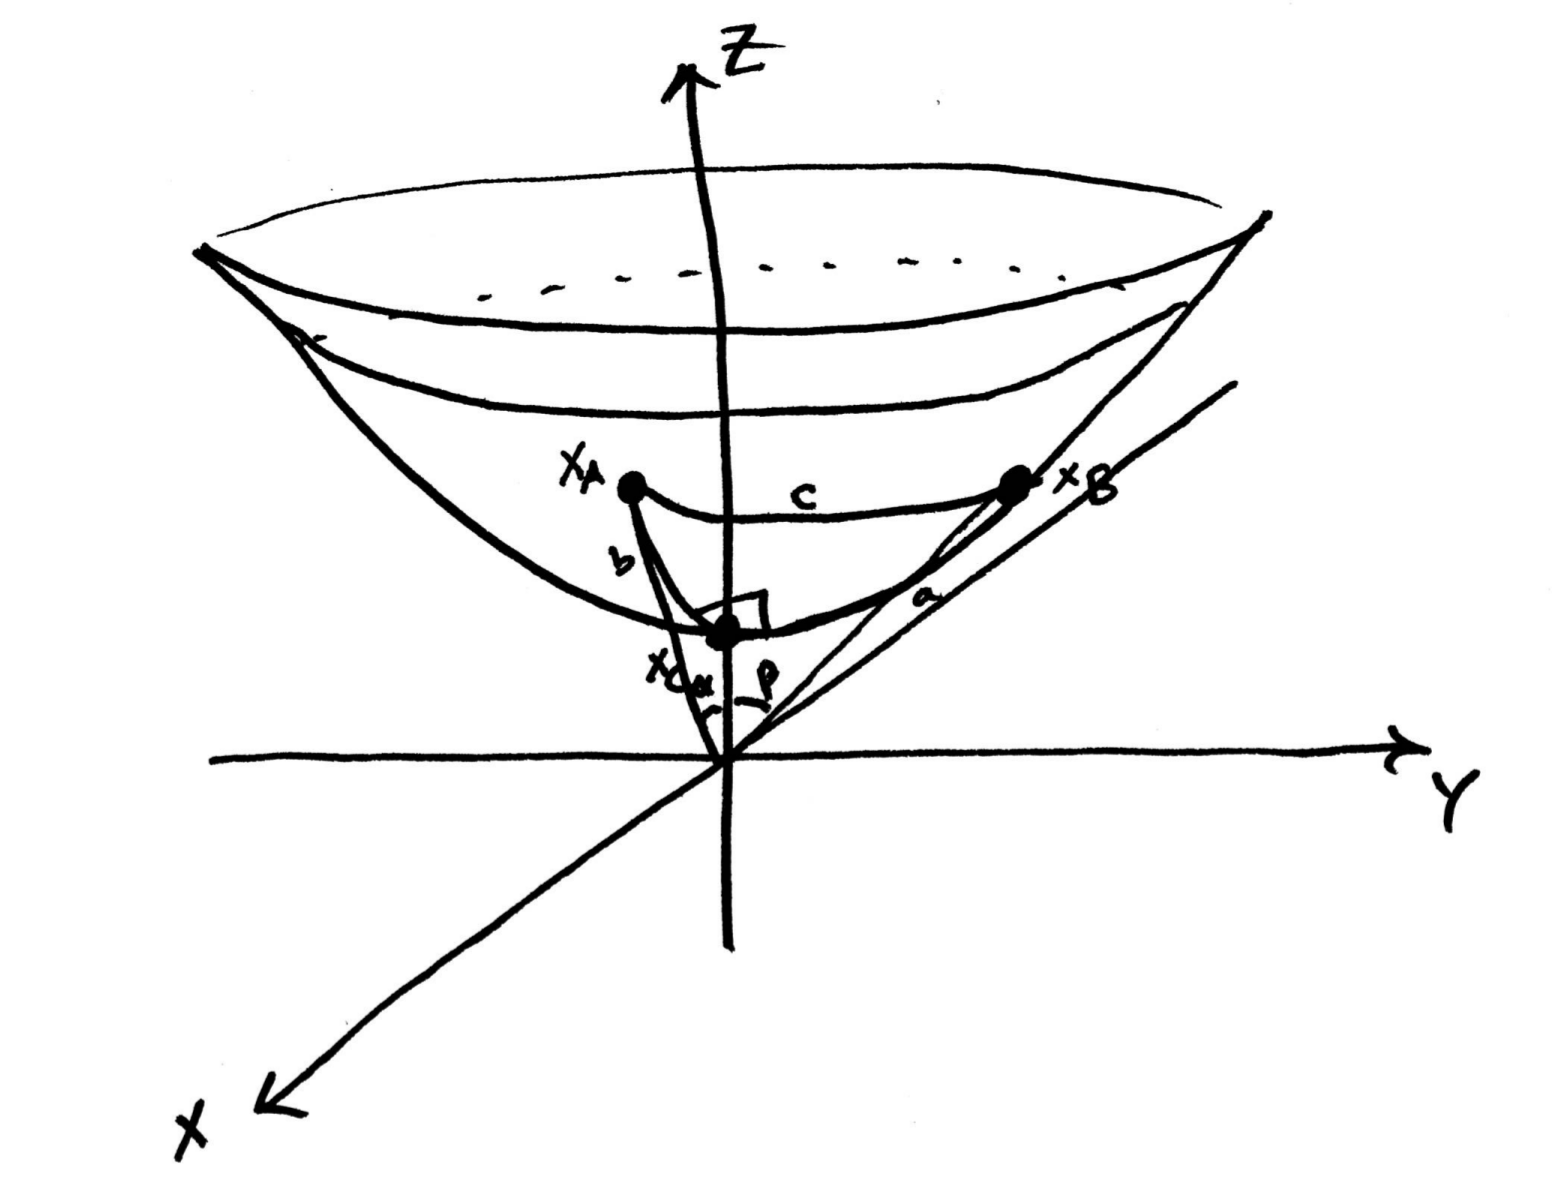
\includegraphics[width=4in]{hypPythag.png}
\end{image}
Hence the length of side $b$ is $|K|^{-1/2}\cdot\alpha$. Using a rigid motion of the form
\[
M_\theta=
\begin{bmatrix}
  \cos\theta & \sin\theta & 0\\
  -\sin\theta & \cos\theta & 0\\
  0 & 0 & 1
\end{bmatrix}
\]
when $\theta = \pi/2$ we see that the length of side $a$ is $|K|^{-1/2}\cdot
\beta$. Set
\[
\gamma = \arccosh\left(\frac{X_A\bullet_K X_B}{|X_A|_K\cdot |X_B|_K}\right).
\]
Since we are working on the $K$-surface,
\begin{align*}
  K^{-1}\cdot \cosh \gamma &= X_A\bullet_K X_B\\
  &=
  \begin{bmatrix}
    |K|^{-1/2}\cdot \sinh\alpha &  0 & \cosh\alpha
  \end{bmatrix}
    \begin{bmatrix}
      1 & 0 & 0\\
      0 & 1 & 0\\
      0 & 0 & K^{-1}
    \end{bmatrix}
    \begin{bmatrix}
      0\\
      |K|^{-1/2}\cdot\sinh\beta\\
      \cosh\beta
    \end{bmatrix}\\
   &=K^{-1} \cdot \cosh\alpha \cdot \cosh\beta.
  \end{align*}
\begin{problem}
  Explain how to progress from the fact that
  \[
  K^{-1}\cdot \cosh \gamma = K^{-1} \cdot \cosh\alpha \cdot \cosh\beta.
  \]
  to the conclusion of the theorem
  \[
  \cosh\left(|K|^{1/2}\cdot c\right)=\cosh\left(|K|^{1/2} \cdot a\right)\cosh\left(|K|^{1/2}\cdot b\right).
  \]
  \begin{freeResponse}
    As we have seen
    \[
    \begin{split}
      |K|^{-1/2}\cdot \alpha &= a,\\
      |K|^{-1/2}\cdot \beta  &= b,\\
      |K|^{-1/2}\cdot \gamma &= c,
    \end{split}
    \qquad\text{so}\qquad
    \begin{split}
      \alpha &= |K|^{1/2} \cdot a,\\
      \beta  &= |K|^{1/2} \cdot b,\\
      \gamma &= |K|^{1/2} \cdot c,\\
    \end{split}
    \]
    and hence
    \[
      \cosh\left(|K|^{1/2}\cdot c\right)=\cosh\left(|K|^{1/2} \cdot a\right)\cosh\left(|K|^{1/2}\cdot b\right).
    \]
  \end{freeResponse}
\end{problem}


\begin{problem}
  Use the Taylor series expansion of $\cos(x)$ centered around $x=0$,
  \[
  \cosh(x) = 1 + \frac{x^2}{2!} + \frac{x^4}{4!} + \frac{x^6}{6!} + \cdots
  \]
to show that for ``small'' triangles, the hyperbolic Pythagorean
Theorem reduces to the euclidean Pythagorean Theorem, meaning
\[
c^2 \approx a^2+b^2.
\]
\begin{freeResponse}
  If
  \[
  \cosh\left(|K|^{1/2}\cdot c\right)=\cosh\left(|K|^{1/2}\cdot a\right)\cosh\left(|K|^{1/2}\cdot b\right),
  \]
  then we may replace each cosine with its Taylor series expansion
  \[
  1 + \frac{\left(|K|^{1/2}\cdot c\right)^2}{2!} + \frac{\left(|K|^{1/2}\cdot c\right)^4}{4!} +  \cdots
  \]
  \[
  =\left(
  1 + \frac{\left(|K|^{1/2}\cdot a\right)^2}{2!} + \frac{\left(|K|^{1/2}\cdot a\right)^4}{4!} +  \cdots
  \right)
  \left(
  1 + \frac{\left(|K|^{1/2}\cdot b\right)^2}{2!} + \frac{\left(|K|^{1/2}\cdot b\right)^4}{4!} + \cdots
  \right).
  \]
  Expanding this out, and discarding higher-order terms (as they will
  go to zero when $a$, $b$, and $c$ are small) we find
  \[
  \frac{-1}{2}\left(|K|^{1/2}\cdot c\right)^2 = \frac{-1}{2}\left(|K|^{1/2}\cdot a\right)^2+\frac{-1}{2}\left(|K|^{1/2}\cdot b\right)^2.
  \]
  Multiplying both sides of the equation by $-2\cdot |K|$, we see that for a
  ``small'' right triangle on the surface of the hyperboloid,
  \[
  c^2 \approx a^2 +b^2.
  \]
\end{freeResponse}
\end{problem}


\begin{problem}
Summarize the results from this section. In particular, indicate which
results follow from the others.
\begin{freeResponse}
\end{freeResponse}
\end{problem}







\end{document}
